\documentclass[a4paper,12pt]{article}
\usepackage{amsmath,amssymb,amsfonts,amsthm}
\usepackage{tikz}
\usepackage [utf8x] {inputenc}
\usepackage [T2A] {fontenc} 
\usepackage[russian]{babel}
\usepackage{cmap} 

% Так ссылки в PDF будут активны
\usepackage[unicode]{hyperref}

% вы сможете вставлять картинки командой \includegraphics[width=0.7\textwidth]{ИМЯ ФАЙЛА}
% получается подключать, как минимум, файлы .pdf, .jpg, .png.
\usepackage{graphicx}
% Если вы хотите явно указать поля:
\usepackage[margin=1in]{geometry}
% Или если вы хотите задать поля менее явно (чем больше DIV, тем больше места под текст):
% \usepackage[DIV=10]{typearea}

\usepackage{fancyhdr}

\newcommand{\bbR}{\mathbb R}%теперь вместо длинной команды \mathbb R (множество вещественных чисел) можно писать короткую запись \bbR. Вместо \bbR вы можете вписать любую строчку букв, которая начинается с '\'.
\newcommand{\eps}{\varepsilon}
\newcommand{\bbN}{\mathbb N}
\newcommand{\dif}{\mathrm{d}}

\newtheorem{Def}{Определение}


\pagestyle{fancy}
\makeatletter % сделать "@" "буквой", а не "спецсимволом" - можно использовать "служебные" команды, содержащие @ в названии
\fancyhead[L]{\footnotesize Термодинамика и молекулярная физика}%Это будет написано вверху страницы слева
\fancyhead[R]{\footnotesize ФМХФ МФТИ}
\fancyfoot[L]{\footnotesize \@author}%имя автора будет написано внизу страницы слева
\fancyfoot[R]{\thepage}%номер страницы —- внизу справа
\fancyfoot[C]{}%по центру внизу страницы пусто

\renewcommand{\maketitle}{%
	\noindent{\bfseries\scshape\large\@title\ \mdseries\upshape}\par
	\noindent {\large\itshape\@author}
	\vskip 2ex}
\makeatother
\def\dd#1#2{\frac{\partial#1}{\partial#2}}


\title{2.2.6 \\ Определение энергии активации по температурной зависимости вязкости жидкости} 
\author{Егор Берсенев} 
\date{27 февраля 2016 г.}

\begin{document}
	\maketitle
	\section{Цель работы}
		\begin{enumerate}
			\item Измерение скорости падения шариков про разной температуре жидкости.
			\item Вычисление вязкости жидкости по закону Стокса и расчёт энергии активации.
		\end{enumerate}
	\section{Оборудование}
		Стеклянный цилиндр, глицерин, термостат, секундомер, горизонтальный компаратор, стеклянные и металлические шарики.
	\section{Теоретическая часть}
		По свойствам жидкости сходны как с газами, так и с твердыми телами. Подобно газам, жидкости принимают форму сосуда, в котором они находятся. Подобно твердым телам, они обладают сравнительно большой плотностью, с трудом поддаются сжатию.
		
		В отличие от твердых тел, жидкости обладают <<рыхлой>> структурой. В них имеются свободные места <<дырки>>, благодаря чему молекулы могут перемещаться, покидая свое место и занимая одну из соседних дырок. Таким образом, молекулы медленно перемещаются внутри жидкости, пребывая часть времени около определенных мест равновесия и образуя картину меняющейся со временем пространственной решетки. На современном языке принято говорить,что в жидкости присутствует ближний, но не дальний порядок,расположение молекул упорядочено в небольших объемах, но порядок перестает замечаться при увеличении расстояния. Для того чтобы перейти в новое состояние,молекула должна преодолеть участки с большой потенциальной энергией, превышающей среднюю тепловую энергию молекул. Для этого тепловая энергия молекул должна вследствие флуктуации увеличиться на некоторую величину $W$, называемую энергией активации. Вследствие этого переходы молекул из одного положения равновесия в другое происходят сравнительно редко и тем реже, чем больше энергия активации.
		В соответствии с формулой Больцмана экспоненциально зависит от $W$. Температурная зависимость вязкости жидкости выражается формулой:
		\begin{equation}
			\eta \sim Ae^{\frac{W}{kT}}
		\end{equation}
		Для определения вязкости в данной работе используется метод Стокса, основанный на измерении скорости свободного падения шарика в жидкости. Сила сопротивления определяется формулой:
		\begin{equation}
			F = -6\pi\eta rv
		\end{equation}
		где $\eta$ --- вязкость жидкости, $v$ --- скорость шарика, $r$ --- его радиус.
		
		Рассмотрим свободное падение шарика в жидкости:
		\begin{equation}
			Vg\left(\rho-\rho_{\text{ж}}\right) - 6\pi\eta rv = V\rho\frac{\dif v}{\dif t}
		\end{equation}
		Решая это уравнение найдем:
		\begin{equation}
			v(t)=v_{\text{уст}}-\left[v_{\text{уст}}-v(0)\right]e^-\frac{t}{\tau}
		\end{equation}
		\begin{equation}
			v_{\text{уст}} = \frac{2}{9}gr^2\frac{\left(\rho-\rho_{\text{ж}}\right)}{\eta}, \qquad \tau = \frac{2}{9}\frac{r^2\rho}{\eta}
		\end{equation}
		Отсюда:
		\begin{equation}
			\eta = \frac{2}{9}gr^2\frac{\rho - \rho_{\text{ж}}}{v_{\text{уст}}}
		\end{equation}
	\section{Устройство установки}
		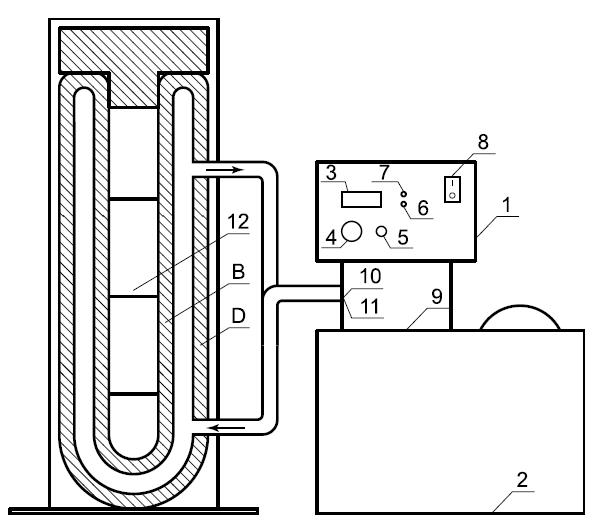
\includegraphics[width = 0.5\linewidth]{instrument}
		\begin{enumerate}
			\item Блок терморегулирования
			\item Ванна
			\item Индикаторное табло
			\item Ручка установки температуры
			\item Кнопка переключения режимов установки температуры
			\item Индикатор уровня жидкости
			\item Индикатор включения нагревателя
			\item Сетевой выключатель прибора
			\item Крышка
			\item Патрубки насоса
			\item Патрубки теплообменника
		\end{enumerate}
	
	
	\section{Ход работы}
		\subsection{Отберем шарики:}
		\begin{center}
			\begin{tabular}{  l |  l  l  l  l  l  l  l  l  l  l }
				\multicolumn{11}{c}{Стеклянные шарики} \\ 
				n.        & 1   & 2   & 3   & 4   & 5  & 6   & 7   & 8   & 9    & 10 \\ \hline
				$d_1$, мм & 2.1 & 2.1 & 2.1 & 2.1 & 2  & 2.1 & 2.1 & 2.1 & 2.05 & 2 \\ \hline
				$d_2$, мм & 2.15 & 2.2 & 2 & 2.1 & 2  & 2.1 & 2.1 & 2.1 & 2.1 & 2 \\ \hline
				$d_3$, мм & 2.1 & 2.15 & 2.1 & 2.2 & 2.1  & 2.1 & 2.05 & 2.1 & 2 & 2 \\ \hline
				$d_1$, мм & 2.1 & 2.15 & 2.1 & 2.1 & 2  & 2.1 & 2.1 & 2.1 & 2.05 & 2 \\ \hline
				\hline
			\end{tabular}
		\end{center}
		\begin{center}
			\begin{tabular}{  l |  l  l  l  l  l  l  l  l  l  l }
				\multicolumn{11}{c}{Металлические шарики} \\ 
				n.        & 1   & 2   & 3   & 4   & 5  & 6   & 7   & 8   & 9    & 10 \\ \hline
				$d_1$, мм & 0.8 & 0.8 & 0.8 & 0.9 & 0.75 & 0.8 & 0.7 & 0.75 & 0.6 & 0.85 \\ \hline
				$d_2$, мм & 0.8 & 0.9 & 0.85 & 0.85 & 0.8  & 0.8 & 0.65 & 0.9 & 0.6 & 0.9 \\ \hline
				$d_3$, мм & 0.85 & 0.9 & 0.8 & 0.85 & 0.8  & 0.9 & 0.65 & 0.85 & 0.6 & 0.9 \\ \hline
				$d_1$, мм & 0.82 & 0.87 & 0.82 & 0.88 & 0.78  & 0.83 & 0.68 & 0.83 & 0.6 & 0.88 \\ \hline
				\hline
			\end{tabular}
		\end{center}
		\subsection{Измерения скорости падения шариков}
		\[
		\frac{\sigma V}{V}=\frac{\sigma T}{T}
		\]
		\begin{center}
			$L = 2S \quad \rho_{\text{ж}} = 1257 \, \text{кг/м}^3$
			
			\begin{tabular}{l  l  l  l  l}
				T, $^oC$ & $1_{\text{с}}$ & $1_{\text{м}}$ & $2_{\text{с}}$ & $2_{\text{м}}$ \\ \hline
				\multicolumn{1}{|c|}{24.5} & 21.87  & 30.37 & 22.28 & 24.62 \\ \hline 
				$V_{\text{уст}}$ & 0.009 & 0.006 & 0.009 & 0.008 \\ \hline
				$\eta \cdot 10^{-3}$, Па$\cdot$c &  0.33 & 0.43 & 0.42 & 0.4 \\ \hline
			\end{tabular}
		\end{center}
		
		\begin{center}
			$L = 2S \quad \rho_{\text{ж}} = 1254 \, \text{кг/м}^3$
			
			\begin{tabular}{l  l  l  l  l}
				T, $^oC$ & $3_{\text{с}}$ & $3_{\text{м}}$ & $4_{\text{с}}$ & $4_{\text{м}}$ \\ \hline
				\multicolumn{1}{|c|}{35.1} & 14.19  & 18.69 & 13.84 & 15.19 \\ \hline
				$V_{\text{уст}}$ & 0.014 & 0.01 & 0.014 & 0.013 \\ \hline
				$\eta \cdot 10^{-3}$, Па$\cdot$c &  0.25 & 0.27 & 0.25 & 0.25 \\ \hline
			\end{tabular}
		\end{center}
		
		\begin{center}
			$L = 2S \quad \rho_{\text{ж}} = 1249 \, \text{кг/м}^3$
			
			\begin{tabular}{l  l  l  l  l}
				T, $^oC$ & $5_{\text{с}}$ & $5_{\text{м}}$ & $6_{\text{с}}$ & $6_{\text{м}}$ \\ \hline
				\multicolumn{1}{|c|}{45.2} & 6.84  & 7.95 & 6.27 & 7.68 \\ \hline
				$V_{\text{уст}}$ & 0.029 & 0.025 & 0.031 & 0.255 \\ \hline
				$\eta \cdot 10^{-3}$, Па$\cdot$c &  0.11 & 0.1 & 0.11 & 0.11 \\ \hline 
			\end{tabular}
		\end{center}
		
		\begin{center}
			$L = S \quad \rho_{\text{ж}} = 1246 \, \text{кг/м}^3$
			
			\begin{tabular}{l  l  l  l  l}
				T, $^oC$ & $7_{\text{с}}$ & $7_{\text{м}}$ & $8_{\text{с}}$ & $8_{\text{м}}$ \\ \hline
				\multicolumn{1}{|c|}{52.1} & 2.38  & 3.97 & 2.63 & 2.53 \\ \hline 
				$V_{\text{уст}}$ & 0.04 & 0.025 & 0.037 & 0.039 \\ \hline
				$\eta \cdot 10^{-3}$, Па$\cdot$c &  0.07 & 0.07 & 0.08 & 0.07 \\ \hline 
			\end{tabular}
		\end{center}
		
		\begin{center}
			$L = S \quad \rho_{\text{ж}} = 1242 \, \text{кг/м}^3$
			
			\begin{tabular}{l  l  l  l  l}
				T, $^oC$ & $9_{\text{с}}$ & $9_{\text{м}}$ & $10_{\text{с}}$ & $10_{\text{м}}$ \\ \hline
				\multicolumn{1}{|c|}{62} & 1.69  & 3.37 & 1.72 & 1.93 \\ \hline 
				$V_{\text{уст}}$ &  0.058 &  0.029 & 0.057 & 0.05 \\ \hline
				$\eta \cdot 10^{-3}$, Па$\cdot$c &  0.05 & 0.04 & 0.05 & 0.05 \\ \hline 
			\end{tabular}
		\end{center}
		
		Проанализируем применимость формулы Стокса в каждом из экспериментов. Во всех опытах к началу измерений тело имело установившуюся скорость, путь релаксации был на порядок меньше пути, пройденного телом до начала измерений.
		
		\subsection{Определение энергии активации}
		\includegraphics[width = 0.9\linewidth]{lnetah1T}
		
		Рассчитаем энергию активации по формуле
		\begin{equation}
			W \sim k\frac{\dif\left(\ln\eta\right)}{\dif\left(1/T\right)}
		\end{equation}
		\[
		W = 1.38\cdot10^{-23}\cdot 6.368 \cdot 10^3 = \left(8.78\pm 0.55\right) \cdot 10^{-20}\, \text{Дж}
		\]
		Табличное значение $W = 8.341 \cdot 10^{-20}\,\text{Дж}$.
		
	
		
	\section{Вывод:}
		Измеряя зависимость вязкости от температуры можно найти энергию активации глицерина.
\end{document}


